\documentclass[12pt]{article}   % artigo fonte 12
\usepackage[
    a4paper,% papel A4
    left=2cm,% margem esquerda
    right=2cm,% margem direita
    top=2cm,% margem superior
    bottom=2cm% margem inferior
]{geometry}
% Caracteres / Acentos / Português do Brasil
\usepackage[utf8]{inputenc}
\usepackage[T1]{fontenc}
\usepackage[brazil]{babel}
\usepackage{ragged2e} %Usar: \justify
% Pacotes Matemática
\usepackage{array,latexsym}
\usepackage{amsmath,amsfonts,amssymb,amsthm,mathabx,amstext}
\usepackage{dsfont}  % Conjuntos: $\mathds{N, Z, Q, R, C}$
% Coloca o nome das tabelas em negrito
\usepackage{caption}
\usepackage{graphicx} % Adiciona suporte a imagens
\usepackage{float}

\begin{document}

\section{Acessibilidade versus cores}

Quando usamos cores em ilustrações estatísticas, devemos nos preocupar em criar
uma paleta de cores que seja acessível para daltônicos. Neste caso, devemos
escolher cores que apresente alto contraste e que não haja sobreposição de cores
que possam dificultar a compreensão da ilustração por daltônicos. Por exemplo,
ao escolher as cores azul e roxo no gráfico à esquerda da Figura
\ref{fig_paleta_azul_branco_roxo}, alguns leitores daltônicos verão tudo azul
como o gráfico à direita da Figura \ref{fig_paleta_azul_branco_roxo}.

\begin{figure}[h!]
    \centering
    \caption{Paleta azul, branco e roxo}
    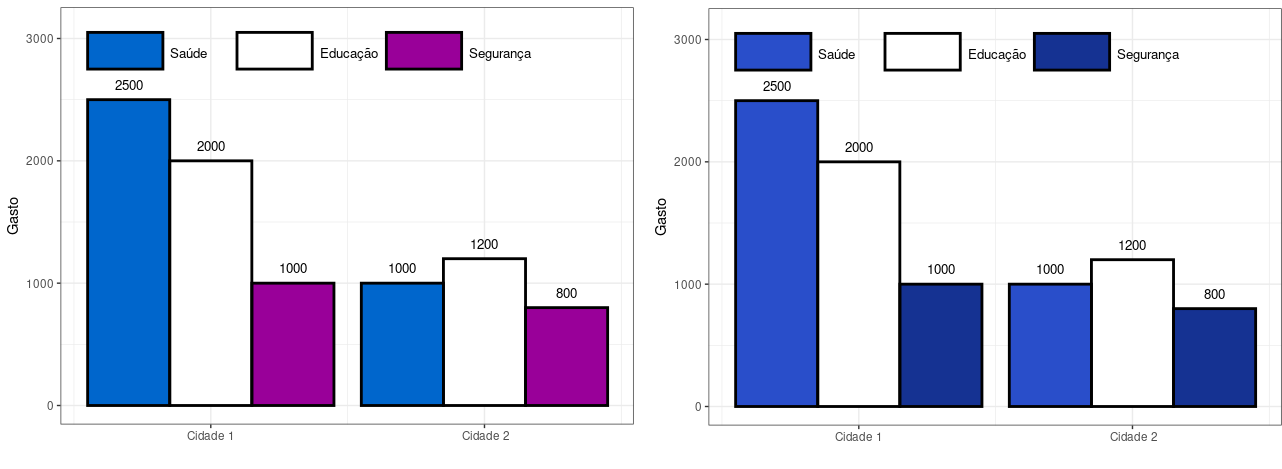
\includegraphics[scale=0.3]{AzulRoxo}
    \label{fig_paleta_azul_branco_roxo}
\end{figure}

O mesmo ocorre com a escolha das cores verde e marrom na Figura 2. Existem
vários tipos de daltonismo, sendo a deuteranopia o caso mais comum de
daltonismo, que atinge 1\% da população masculina. Quem tem deuteranopia
confunde verde, amarelo, vermelho e marrom, bem como, azul, roxo, azul água e
rosa. Este é o problema na escolha da paleta de cores nas Figuras
\ref{fig_paleta_azul_branco_roxo} e \ref{fig_verde_branco_marrom}.

\begin{figure}[h!]
    \centering
    \caption{Paleta verde, branco e marrom}
    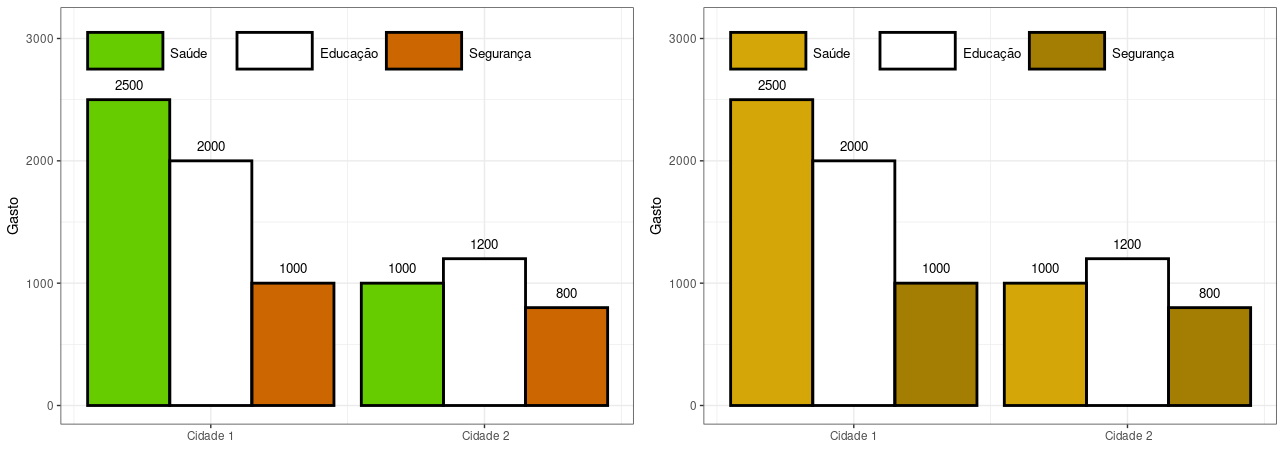
\includegraphics[scale=0.3]{VerdeMarrom}
    \label{fig_verde_branco_marrom}
\end{figure}

Para entender melhor o problema, vamos considerar os casos mais comum de
daltonismo (informações obtidas da Wikipédia):

\begin{itemize}
    \item \textbf{protanopia}, quando há ausência na retina de cones
    ``vermelhos'', resultando na impossibilidade de discriminar cores no
    segmento verde-amarelo-vermelho do espectro.
    
    \item \textbf{deuteranopia}, quando há ausência de cones ``verdes'',
    resultando, igualmente, na impossibilidade de discriminar cores no segmento
    verde-amarelo-vermelho do espectro.
    
    \item \textbf{tritanopia}, quando há ausência de cones ``azuis'', resultando
    na impossibilidade de ver cores na faixa azul-amarelo.
\end{itemize}

\begin{figure}
    \centering
    \caption{Paleta com cores reais e como é vista por daltônicos}
    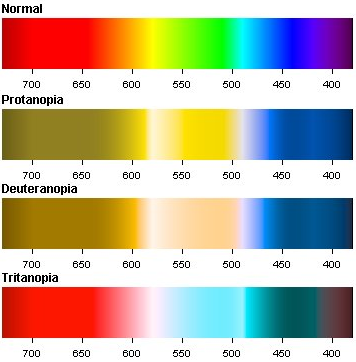
\includegraphics[scale=1.3]{paleta}
    \label{fig_paleta_daltonicos}
    \vspace{1cm}
\end{figure}

\begin{figure}
    \centering
    \caption{Paleta azul, branco e laranja}
    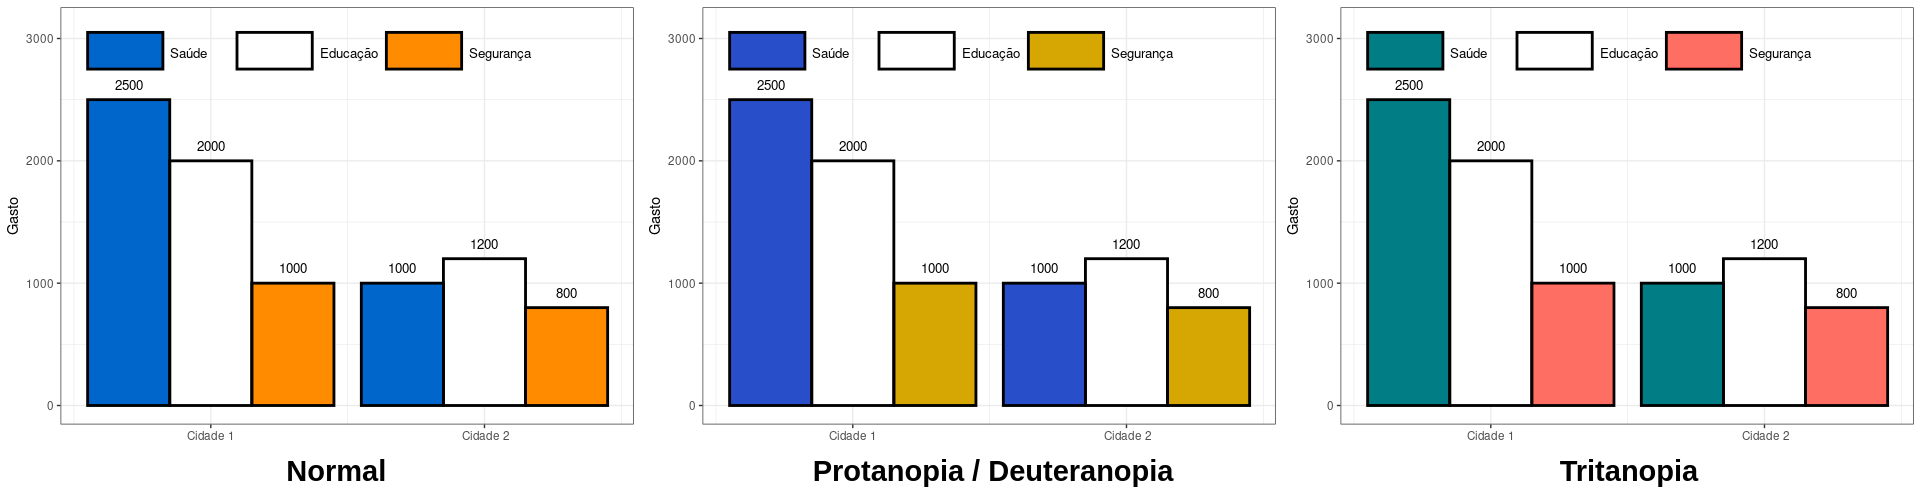
\includegraphics[scale=0.3]{AzulLaranja}
    \label{fig_paleta_azul_branco_laranja}
\end{figure}

Na Figura \ref{fig_paleta_daltonicos}, temos o espectro de cores normal
(primeira faixa) e como essas cores são vistas por daltônicos com protanopia
(segunda faixa), deuteranopia (terceira faixa) e tritanopia (quarta faixa). O
caso mais grave e raro é a monocromacia, que ocorre quando o indivíduo apenas
percebe a luminosidade, ou seja, ver apenas em uma escala de tons de cinza.
\par Portanto, devemos tomar cuidado ao criar uma paleta de cores para gráficos.
Um exemplo que funciona é o da Figura \ref{fig_paleta_azul_branco_laranja}. O
recomendado é, sempre que possível, escolher uma cor na faixa que é vista como
amarelo/vermelho pelos daltônicos e outra na faixa que é vista como
azul/turquesa(azul água) para garantir o contraste.
\par O ponto crucial na questão do uso de cores é que, por mais que criemos uma
paleta de cores com bom contraste para todos os tipos de daltonismo, ainda
estamos usando cores. Quem tem daltonismo não consegue distinguir as cores por
seus nomes e portanto, ao se referir no texto pelo nome da cor que está na
figura, o daltônico provavelmente não vai entender. Portanto, a solução mais
acessível é não confiar nas cores para seus trabalhos e projetos, mas sim, usar
padrões. Pontos, traços em várias direções, larguras e espaçamentos, formas
geométricas, símbolos e texturas passam a mesma informação e sem confundir
daltônicos. Além disso, nada impede de usarmos cores quando também usamos
padrões, como é o caso dos gráficos da Figura \ref{fig_padroes}.

\begin{figure}[h!]
    \centering
    \caption{Exemplo de uso de padrões}
    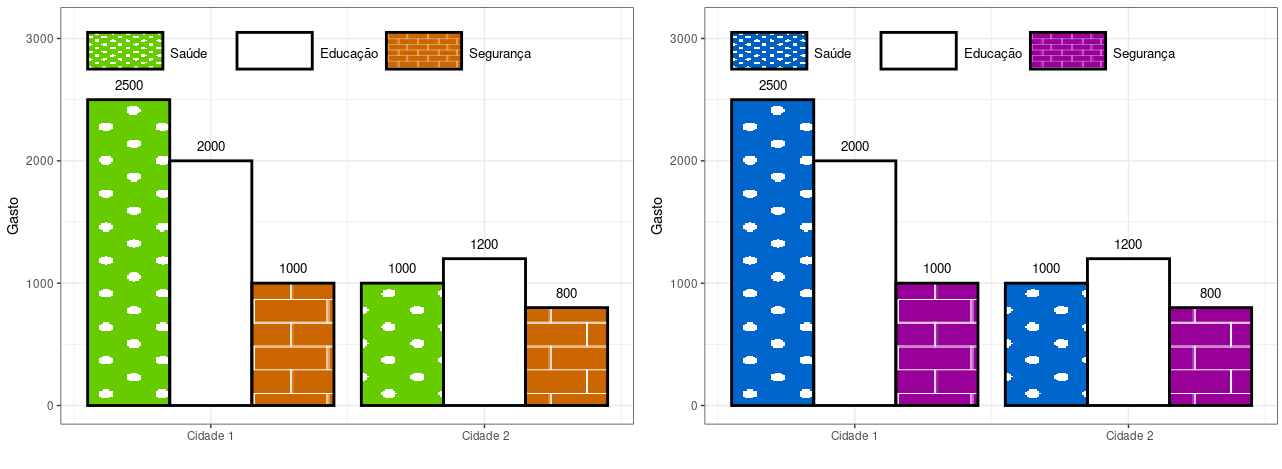
\includegraphics[scale=0.3]{padrao}
    \label{fig_padroes}
\end{figure}

\end{document}

